% ============================================================
%  يُترجَم بـ XeLaTeX  (في Overleaf: Menu → Compiler → XeLaTeX)
%  الخط: Amiri (متوفر في Overleaf، أو حمّله من github.com/aliftype/amiri)
% ============================================================
\documentclass[12pt,a4paper]{article}
\usepackage[a4paper,margin=1.7cm,top=2.3cm,bottom=2.9cm,headheight=15pt,footskip=1.5cm]{geometry}
\usepackage{amsmath,amssymb}
\usepackage{icomma}
\usepackage[english,bidi=default,layout=lists]{babel}
\babelprovide[import,main]{arabic}
\babelfont{rm}[Scale=1.08]{Amiri}
\babelfont{sf}[Scale=1.08]{Amiri}
\usepackage[most]{tcolorbox}
\usepackage{tikz}
\usetikzlibrary{arrows.meta,calc,shadings}
\usepackage{array}
\usepackage{colortbl}
\usepackage{fancyhdr}
\usepackage{titlesec}
\usepackage{enumitem}
\usepackage{collcell}
\usepackage{needspace}
\usepackage{etoolbox}
\newcolumntype{C}{>{\collectcell\ar}c<{\endcollectcell}}
\pretocmd{\section}{\Needspace{15\baselineskip}}{}{}
\pretocmd{\subsection}{\Needspace{11\baselineskip}}{}{}

\definecolor{cDef}{HTML}{1F4E9C}
\definecolor{cThm}{HTML}{B3261E}
\definecolor{cRem}{HTML}{2E7D32}
\definecolor{cEx}{HTML}{C76B00}
\definecolor{cMeth}{HTML}{6A1B9A}
\definecolor{cSol}{HTML}{00695C}
\definecolor{cSec}{HTML}{1F3A68}

\titleformat{\section}{\Large\bfseries\color{cSec}}{\thesection.}{0.6em}{}[{\color{cSec!60}\titlerule[1pt]}]
\titleformat{\subsection}{\large\bfseries\color{cThm!85!black}}{\thesubsection.}{0.5em}{}
\titlespacing*{\section}{0pt}{14pt}{8pt}
\titlespacing*{\subsection}{0pt}{10pt}{5pt}
\setlength{\parindent}{0pt}
\setlength{\parskip}{4pt}
\setlist{itemsep=2pt,topsep=3pt}

\newtcolorbox{arbox}[3][]{enhanced,
  colback=#2!5,colframe=#2!80!black,arc=2mm,boxrule=0.8pt,
  left=6pt,right=6pt,top=8pt,bottom=5pt,
  fonttitle=\bfseries,coltitle=white,
  title={\foreignlanguage{arabic}{#3}},
  attach boxed title to top right={xshift=-5mm,yshift=-3mm},
  boxed title style={colback=#2!80!black,arc=1.5mm,boxrule=0pt},
  before upper={\selectlanguage{arabic}},
  before skip=8pt,after skip=8pt,breakable,#1}
\newenvironment{BOX}[2]{\begin{otherlanguage}{english}\begin{arbox}{#1}{#2}}{\end{arbox}\end{otherlanguage}}
\newenvironment{tarif}[1][تعريف]{\begin{BOX}{cDef}{#1}}{\end{BOX}}
\newenvironment{khassia}[1][خاصية]{\begin{BOX}{cThm}{#1}}{\end{BOX}}
\newenvironment{molahada}[1][ملاحظة]{\begin{BOX}{cRem}{#1}}{\end{BOX}}
\newenvironment{mithal}[1][مثال]{\begin{BOX}{cEx}{#1}}{\end{BOX}}
\newenvironment{tariqa}[1][طريقة]{\begin{BOX}{cMeth}{#1}}{\end{BOX}}

\newcounter{exo}
\newenvironment{tamrin}[1]{\stepcounter{exo}\begin{BOX}{cSec}{التمرين \theexo: #1}}{\end{BOX}}
\newenvironment{hal}{\Needspace{12\baselineskip}\begin{otherlanguage}{english}\begin{arbox}[breakable]{cSol}{حل التمرين \theexo}}{\end{arbox}\end{otherlanguage}}

\newenvironment{LTR}{\begin{otherlanguage}{english}}{\end{otherlanguage}}
\newcommand{\ar}[1]{\foreignlanguage{arabic}{#1}}

\renewcommand{\dots}{\mathinner{\ldotp\ldotp\ldotp}}
\renewcommand{\ldots}{\mathinner{\ldotp\ldotp\ldotp}}
\renewcommand{\cdots}{\mathinner{\cdotp\cdotp\cdotp}}
\newcommand{\N}{\mathbb{N}}
\newcommand{\Z}{\mathbb{Z}}
\newcommand{\D}{\mathbb{D}}
\newcommand{\Q}{\mathbb{Q}}
\newcommand{\R}{\mathbb{R}}
\newcommand{\pgcd}{\operatorname{PGCD}}
\newcommand{\ppcm}{\operatorname{PPCM}}

% \NLseg{a}{b}{[}{]} ; \NLright{a}{[} ; \NLleft{b}{]}  (interval on a number line)
\newcommand{\NLseg}[4]{\begin{LTR}\begin{tikzpicture}[baseline=-0.6ex]
 \draw[-{Stealth[length=2mm]},gray!70](0,0)--(3.4,0);
 \draw[line width=2pt,cThm!80!black](0.7,0)--(2.7,0);
 \node[cThm!80!black,font=\LARGE] at (0.7,0){$#3$};
 \node[cThm!80!black,font=\LARGE] at (2.7,0){$#4$};
 \node[below=3pt,font=\footnotesize] at (0.7,0){$#1$};
 \node[below=3pt,font=\footnotesize] at (2.7,0){$#2$};
\end{tikzpicture}\end{LTR}}
\newcommand{\NLright}[2]{\begin{LTR}\begin{tikzpicture}[baseline=-0.6ex]
 \draw[-{Stealth[length=2mm]},gray!70](0,0)--(3.4,0);
 \draw[line width=2pt,cThm!80!black](1.3,0)--(3.3,0);
 \node[cThm!80!black,font=\LARGE] at (1.3,0){$#2$};
 \node[below=3pt,font=\footnotesize] at (1.3,0){$#1$};
\end{tikzpicture}\end{LTR}}
\newcommand{\NLleft}[2]{\begin{LTR}\begin{tikzpicture}[baseline=-0.6ex]
 \draw[-{Stealth[length=2mm]},gray!70](0,0)--(3.4,0);
 \draw[line width=2pt,cThm!80!black](0.05,0)--(2.1,0);
 \node[cThm!80!black,font=\LARGE] at (2.1,0){$#2$};
 \node[below=3pt,font=\footnotesize] at (2.1,0){$#1$};
\end{tikzpicture}\end{LTR}}

% ---------- social-media icons (pure TikZ) ----------
\definecolor{cFB}{HTML}{1877F2}
\definecolor{cTG}{HTML}{229ED9}
\definecolor{cIG1}{HTML}{FEDA75}
\definecolor{cIG2}{HTML}{D62976}
\definecolor{cIG3}{HTML}{4F5BD5}
\newcommand{\fbicon}{\begin{LTR}\begin{tikzpicture}[baseline=-0.75ex,x=1em,y=1em]
 \fill[cFB] (0,0) circle (0.55);
 \node[white,inner sep=0,font=\usefont{TU}{lmss}{bx}{n}\small] at (0.04,-0.02) {f};
\end{tikzpicture}\end{LTR}}
\newcommand{\igicon}{\begin{LTR}
\begin{tikzpicture}[baseline=-0.75ex,x=1em,y=1em]
 \shade[lower left=cIG1,lower right=cIG2,upper left=cIG2,upper right=cIG3,rounded corners=0.28em] (-0.55,-0.55) rectangle (0.55,0.55);
 \draw[white,line width=0.09em,rounded corners=0.18em] (-0.36,-0.36) rectangle (0.36,0.36);
 \draw[white,line width=0.09em] (0,0) circle (0.17);
 \fill[white] (0.22,0.22) circle (0.05);
\end{tikzpicture}\end{LTR}}
\newcommand{\tgicon}{\begin{LTR}
\begin{tikzpicture}[baseline=-0.75ex,x=1em,y=1em]
 \fill[cTG] (0,0) circle (0.55);
 \fill[white] (-0.33,0.0) -- (0.32,0.27) -- (0.2,-0.3) -- (0.0,-0.15) -- (-0.08,-0.28) -- (-0.08,-0.08) -- cycle;
 \fill[cTG!70!black] (-0.08,-0.08) -- (0.25,0.2) -- (0.0,-0.15) -- (-0.08,-0.28) -- cycle;
\end{tikzpicture}\end{LTR}}
% page number: black box, white two-digit number, at the right of the social row
\newcommand{\PageBox}{\begin{LTR}\tikz[baseline=(p.base)]\node[fill=black,text=white,inner sep=2.5pt,minimum width=1.6em,minimum height=1.3em,font=\usefont{TU}{lmss}{bx}{n}\small](p){\ifnum\value{page}<10 0\fi\arabic{page}};\end{LTR}}
% visual left-to-right order: Telegram | Instagram | Facebook | page box
\newcommand{\SocialRow}{\begin{otherlanguage}{english}%
 \ar{\textbf{الأستاذ سوايسية هشام للرياضيات}}\ \tgicon\hfill
 \textbf{prof\_hicham\_math}\ \igicon\hfill
 \ar{\textbf{الأستاذ سوايسية هشام للرياضيات}}\ \fbicon\hspace{2.2em}\PageBox\end{otherlanguage}}

\pagestyle{fancy}
\fancyhf{}
\renewcommand{\headrulewidth}{0.6pt}
\renewcommand{\footrulewidth}{0.4pt}
% \SetHeader{right head: document title}{left head: level -- stream}
\newcommand{\SetHeader}[2]{%
 \fancyhead[C]{\parbox{\textwidth}{\ar{#1\hfill #2}}}%
 \fancyfoot[C]{\parbox{\textwidth}{\small\SocialRow}}}
\usepackage{tkz-tab}
\usepackage{multicol}
% variation / sign table (LTR)
\newenvironment{TAB}{\par\begin{center}\begin{LTR}\begin{tikzpicture}[scale=0.95,every node/.style={font=\small}]}{\end{tikzpicture}\end{LTR}\end{center}}
% grid + axes, clipped: \begin{GR}{xmin}{xmax}{ymin}{ymax}{unit cm}
\newenvironment{GR}[5]{\par\begin{center}\begin{LTR}\begin{tikzpicture}[x=#5cm,y=#5cm,font=\footnotesize]
 \draw[gray!25,very thin] (#1,#3) grid (#2,#4);
 \draw[-{Stealth[length=2mm]}] (#1,0)--(#2+0.3,0) node[below left]{$x$};
 \draw[-{Stealth[length=2mm]}] (0,#3)--(0,#4+0.3) node[below left]{$y$};
 \node[below left] at (0,0){$O$};
 \begin{scope}\clip (#1,#3) rectangle (#2,#4);}
{\end{scope}\end{tikzpicture}\end{LTR}\end{center}}
\newcommand{\Ticks}[2]{\foreach \t in {#1} \node[below,font=\scriptsize] at (\t,0){$\t$}; \foreach \t in {#2} \node[left,font=\scriptsize] at (0,\t){$\t$};}
\newcommand{\bx}[1]{\ensuremath{\colorbox{cDef!12}{$\displaystyle #1$}}}
\newcommand{\TwoCol}[4]{\par\begin{LTR}\noindent\begin{minipage}[t]{#1\textwidth}\selectlanguage{arabic}#2\end{minipage}\hfill\begin{minipage}[t]{#3\textwidth}\selectlanguage{arabic}#4\end{minipage}\end{LTR}\par}
\newcommand{\RL}[4]{\TwoCol{#3}{#4}{#1}{#2}}  % \RL{w1}{right content}{w2}{left content}
\newcommand{\ok}{$\textcolor{cRem}{\checkmark}$}
\newcommand{\limn}{\displaystyle\lim_{n\to+\infty}}
% sub-questions, each on its own line
\newenvironment{sq}{\begin{itemize}[leftmargin=2.4em,itemsep=3pt]}{\end{itemize}}
\newcommand{\qa}{\item[(أ)]}\newcommand{\qb}{\item[(ب)]}\newcommand{\qc}{\item[(جـ)]}\newcommand{\qd}{\item[(د)]}\newcommand{\qe}{\item[(هـ)]}
\newcommand{\pa}{\par\smallskip\textbf{(أ)} }\newcommand{\pb}{\par\smallskip\textbf{(ب)} }\newcommand{\pc}{\par\smallskip\textbf{(جـ)} }\newcommand{\pd}{\par\smallskip\textbf{(د)} }\newcommand{\pe}{\par\smallskip\textbf{(هـ)} }
\newcommand{\QQ}[1]{\par\smallskip\textbf{#1.} }
\newenvironment{tmr}{\stepcounter{exo}\begin{BOX}{cSec}{تمرين محلول \theexo}}{\end{BOX}}
\newcommand{\ABC}[3]{\\[2pt]\begin{tabular}{p{0.28\textwidth}p{0.28\textwidth}p{0.28\textwidth}}(جـ) \ #3 & (ب) \ #2 & (أ) \ #1\end{tabular}}
\pretocmd{\section}{\Needspace{24\baselineskip}}{}{}
\newtcbox{\bxtbox}{on line,colback=cDef!12,colframe=cDef!12,boxrule=0pt,arc=1pt,boxsep=0pt,left=2pt,right=2pt,top=1pt,bottom=1pt}
\newcommand{\bxt}[1]{\foreignlanguage{english}{\bxtbox{\ar{#1}}}}
\usepackage{longtable}
\setlength{\LTpre}{4pt}\setlength{\LTpost}{0pt}
\newcommand{\Phase}[1]{\textbf{#1}}
\newcommand{\Fld}[2]{\textbf{#1:}\ #2}
% رأس المذكرة على نمط النموذج: إطار بعنوان «مذكرة رقم»، معلومات الحصة، ثم إطار الكفاءات
\newcommand{\ModhHead}[9]{%
\begin{LTR}
\begin{tcolorbox}[enhanced,colback=white,colframe=cThm!85!black,arc=4mm,boxrule=1pt,top=14pt,bottom=6pt,left=8pt,right=8pt,
 overlay={\node[fill=cThm!85!black,text=white,rounded corners=3mm,inner xsep=14pt,inner ysep=4pt,font=\large\bfseries] at ([yshift=0pt]frame.north){\ar{مذكرة رقم #1}};},
 before upper={\selectlanguage{arabic}}]
\begin{tabular}{@{}p{0.4\linewidth}p{0.55\linewidth}@{}}
\Fld{المستوى}{#2} & \Fld{الثانوية}{\dotfill}\\[3pt]
\Fld{المادة}{رياضيات} & \Fld{ميدان التعلم}{#3}\\[3pt]
\Fld{المدة}{#5} & \Fld{الوحدة التعلمية}{#4}\\[3pt]
\Fld{الأستاذ}{\dotfill} & \Fld{المحتوى المعرفي}{#6}\\
\end{tabular}
\end{tcolorbox}
\begin{tcolorbox}[enhanced,colback=white,colframe=cThm!85!black,arc=3mm,boxrule=0.8pt,sidebyside,sidebyside align=top,lefthand ratio=0.5,
 segmentation style={dashed,cThm!60},before upper={\selectlanguage{arabic}},before lower={\selectlanguage{arabic}}]
\textbf{الكفاءات المستهدفة:}\par #8
\tcblower
\textbf{الكفاءات القبلية:}\par #7
\end{tcolorbox}
\end{LTR}
\par\smallskip\textbf{الوسائل:} #9\par\smallskip}
\newenvironment{Sayr}{%
\begin{LTR}\renewcommand{\arraystretch}{1.25}
\begin{longtable}{|p{0.17\textwidth}|>{\centering\arraybackslash}p{0.06\textwidth}|p{0.53\textwidth}|>{\centering\arraybackslash}p{0.12\textwidth}|}
\hline\rowcolor{cThm!12}\ar{\textbf{توجيهات وتعاليق}} & \ar{\textbf{المدة}} & \ar{\textbf{سير الحصة}} & \ar{\textbf{مراحل الحصة}}\\\hline\endhead
\hline\endfoot}{\end{longtable}\end{LTR}}
% سطر في الجدول: \Row{مرحلة}{سير}{مدة}{توجيهات}
\newcommand{\Row}[4]{\ar{\small #4} & \ar{#3} & \ar{#2} & \cellcolor{cThm!8}\ar{\Phase{#1}}\\\hline}

\newcommand{\Lab}[2]{\foreignlanguage{english}{\tcbox[on line,colback=#1,colframe=#1,boxrule=0pt,arc=2pt,boxsep=1pt,left=5pt,right=5pt,top=1pt,bottom=1pt]{\ar{\textcolor{white}{\textbf{#2}}}}}}
\newcommand{\Num}[1]{\foreignlanguage{english}{\tikz[baseline=(c.base)]\node[fill=cDef,text=white,inner sep=2pt,font=\footnotesize\bfseries](c){#1};}}
\newcommand{\ck}{\ensuremath{{\color{cRem}\checkmark}}}
\newenvironment{Kad}[1]{\par\smallskip\Lab{#1}}{\par}
\SetHeader{\small\bfseries\color{cSec}مذكرات محور: الزوايا الموجهة وحساب المثلثات}{\small\color{cSec}السنة الثانية ثانوي -- علوم تجريبية}
\begin{document}
\begin{LTR}
\begin{tcolorbox}[enhanced,colback=cThm!85!black,colframe=cThm!85!black,arc=3mm,halign=center,boxrule=0pt,top=12pt,bottom=12pt,before upper={\selectlanguage{arabic}}]
{\color{white}\fontsize{24}{30}\selectfont\bfseries مذكرات محور: الزوايا الموجهة وحساب المثلثات}\\[8pt]
{\color{white}\large السنة الثانية ثانوي -- علوم تجريبية (صالحة لشعبتي رياضيات وتقني رياضي)}\\[4pt]
{\color{white}\large 6 مذكرات (12 ساعة) -- السنة الدراسية 2026-2027}
\end{tcolorbox}
\end{LTR}
\begin{BOX}{cThm}{يتضمن هذا العمل}
\begin{enumerate}[label=\textbf{مذكرة \arabic{enumi}:},leftmargin=6em,start=37]
\item الراديان والزاوية الموجهة لشعاعين ، القيس الرئيسي.
\item خواص الزوايا الموجهة.
\item حساب المثلثات: جيب التمام والجيب.
\item جيب تمام وجيب الزوايا المرفقة (دساتير التحويل).
\item المعادلات المثلثية الأساسية.
\item المتراجحات المثلثية البسيطة.
\end{enumerate}
مراجع النشاطات والتمارين: الكتاب المدرسي للسنة الثانية ثانوي (باب الزوايا الموجهة ص 210--211 ، أعمال موجهة ص 222). دساتير الجمع تأتي في محور الجداء السلمي.
\end{BOX}
\newpage
\ModhHead{37}{2 ع ت}{هندسة}{الزوايا الموجهة وحساب المثلثات}{02 سا}{الراديان والزاوية الموجهة لشعاعين ، القيس الرئيسي}%
{\begin{itemize}\item الدائرة المثلثية ، الراديان (1 ج م).\end{itemize}}%
{\begin{itemize}\item تعيين أقياس زاوية موجهة لشعاعين وقيسها الرئيسي.\end{itemize}}%
{المنهاج ، الكتاب المدرسي ، مراجع ، الحاسبة ، أدوات الهندسة.}
\begin{Sayr}
\Row{مرحلة الانطلاق}{%
\textbf{التهيئة النفسية:} عقارب الساعة تدور في اتجاه: هل الدوران من $12$ إلى $3$ هو نفسه من $3$ إلى $12$ ؟}{10 د}{مثال الساعة.}
\Row{التشخيص والاكتشاف}{%
\Lab{cEx}{مناقشة النشاطين 01 صفحة 210 و 03 صفحة 211}\par\ck\ جدول التناسبية بين الدرجة والراديان: $180^\circ\leftrightarrow\pi$ rad.\par
\ck\ نقطتان على الدائرة الموجهة: طول القوس من الأولى إلى الثانية في الاتجاه الموجب يعطي قيساً للزاوية الموجهة.\par
}{35 د}{جدول التناسبية.}
\Row{بناء المعارف}{%
\Lab{cDef}{تعريف}\ $\vec u$ و $\vec v$ شعاعان غير معدومين: للزاوية الموجهة $(\vec u;\vec v)$ أقياس لا نهائية ، إذا كان $\alpha$ أحدها فكل أقياسها $\alpha+2k\pi$ ($k\in\mathbb Z$) ، ونكتب $(\vec u;\vec v)=\alpha\ [2\pi]$.\par\Lab{cDef}{القيس الرئيسي}\ القيس الوحيد الذي ينتمي إلى $]-\pi;\pi]$.\par}{50 د}{نرسم على الدائرة المثلثية.}
\Row{}{%
\Lab{cMeth}{طريقة}\ نطرح أو نضيف مضاعفات $2\pi$: نكتب البسط على شكل قسمة إقليدية.\par\Lab{cEx}{مثال}\ $\dfrac{29\pi}6=\dfrac{5\pi}6+4\pi$: القيس الرئيسي $\dfrac{5\pi}6$ ؛ $-\dfrac{17\pi}4=-\dfrac\pi4-4\pi$: القيس الرئيسي $-\dfrac\pi4$.\par}{}{}
\Row{}{%
\Lab{cThm!80!black}{حذار}\ $(\vec u;\vec v)$ و $(\vec v;\vec u)$ مختلفتان: الترتيب مهم.}{}{}
\Row{التقويم}{%
\Lab{cEx}{تطبيق}\par عيّن القيس الرئيسي لكل من: $\dfrac{37\pi}3$ ، $-\dfrac{11\pi}6$ ، $\dfrac{7\pi}2$.\par\textbf{الحل:} $\dfrac{37\pi}3=\dfrac\pi3+12\pi$: $\dfrac\pi3$ ؛ $-\dfrac{11\pi}6=\dfrac\pi6-2\pi$: $\dfrac\pi6$ ؛ $\dfrac{7\pi}2=-\dfrac\pi2+4\pi$: $-\dfrac\pi2$.\par\textbf{واجب منزلي:} تمارين 18 ، 19 ، 20 ، 25 ، 26 ، 28 من باب الزوايا الموجهة.\par\smallskip\textbf{ملاحظات حول سير الحصة:} \dotfill}{25 د}{تقويم فردي.}
\end{Sayr}
\newpage
\ModhHead{38}{2 ع ت}{هندسة}{الزوايا الموجهة وحساب المثلثات}{02 سا}{خواص الزوايا الموجهة}%
{\begin{itemize}\item الزاوية الموجهة ، القيس الرئيسي.\end{itemize}}%
{\begin{itemize}\item استعمال خواص الزوايا الموجهة (علاقة شال) لإثبات تقايس زوايا واستقامية نقط.\end{itemize}}%
{المنهاج ، الكتاب المدرسي ، مراجع ، الحاسبة ، أدوات الهندسة.}
\begin{Sayr}
\Row{مرحلة الانطلاق}{%
\textbf{التهيئة النفسية:} إذا دار شعاع بزاوية $\frac\pi3$ ثم بزاوية $\frac\pi6$ ، فبكم دار إجمالاً؟}{10 د}{سؤال ذهني.}
\Row{التشخيص والاكتشاف}{%
\Lab{cEx}{وضعية مقترحة}\ $ABC$ مثلث متقايس الأضلاع مباشر.\par\ck\ $(\overrightarrow{AB};\overrightarrow{AC})=\frac\pi3$ ؛ ما قيس $(\overrightarrow{AC};\overrightarrow{AB})$ ؟ و $(\overrightarrow{AB};\overrightarrow{CA})$ ؟\par
}{35 د}{الشكل على السبورة.}
\Row{بناء المعارف}{%
\Lab{cThm}{خاصية}\ من أجل أشعة غير معدومة:\par\ck\ \textbf{علاقة شال}: $(\vec u;\vec v)+(\vec v;\vec w)=(\vec u;\vec w)\ [2\pi]$.\par
\ck\ $(\vec v;\vec u)=-(\vec u;\vec v)$ ؛ $(-\vec u;\vec v)=(\vec u;\vec v)+\pi$ ؛ $(-\vec u;-\vec v)=(\vec u;\vec v)$.\par
\ck\ $\vec u$ و $\vec v$ مرتبطان خطياً إذا وفقط إذا كان $(\vec u;\vec v)=0$ أو $\pi\ [2\pi]$.\par
\Lab{cEx}{مثال}\ مع الوضعية: $(\overrightarrow{AC};\overrightarrow{AB})=-\frac\pi3$ ؛ $(\overrightarrow{AB};\overrightarrow{CA})=(\overrightarrow{AB};\overrightarrow{AC})+\pi=\frac{4\pi}3=-\frac{2\pi}3\ [2\pi]$.\par}{50 د}{نلون الأشعة.}
\Row{}{%
\Lab{cRem}{ملاحظات}\ لإثبات استقامية $A$ ، $B$ ، $C$ نبين أن $(\overrightarrow{AB};\overrightarrow{AC})=0$ أو $\pi\ [2\pi]$.\par\Lab{cThm!80!black}{حذار}\ عند تغيير اتجاه شعاع واحد نضيف $\pi$.}{}{}
\Row{التقويم}{%
\Lab{cEx}{تطبيق}\par $ABCD$ مربع مباشر. عيّن القيس الرئيسي لـ $(\overrightarrow{AB};\overrightarrow{CD})$ و $(\overrightarrow{DA};\overrightarrow{AB})$.\par\textbf{الحل:} $\overrightarrow{CD}=-\overrightarrow{AB}$: $\pi$ ؛ $(\overrightarrow{DA};\overrightarrow{AB})=(\overrightarrow{AD};\overrightarrow{AB})+\pi=-\frac\pi2+\pi=\frac\pi2$.\par\textbf{واجب منزلي:} تمرينا 30 و 31 من باب الزوايا الموجهة.\par\smallskip\textbf{ملاحظات حول سير الحصة:} \dotfill}{25 د}{تقويم فردي.}
\end{Sayr}
\newpage
\ModhHead{39}{2 ع ت}{هندسة}{الزوايا الموجهة وحساب المثلثات}{02 سا}{حساب المثلثات: جيب التمام والجيب}%
{\begin{itemize}\item الدائرة المثلثية ، cos و sin (1 ج م).\end{itemize}}%
{\begin{itemize}\item استعمال القيم الشهيرة والعلاقة $\cos^2x+\sin^2x=1$.\end{itemize}}%
{المنهاج ، الكتاب المدرسي ، مراجع ، الحاسبة ، أدوات الهندسة.}
\begin{Sayr}
\Row{مرحلة الانطلاق}{%
\textbf{التهيئة النفسية:} ما إحداثيا النقطة المرفقة بالعدد $\frac\pi2$ على الدائرة المثلثية؟ وبالعدد $\pi$ ؟}{10 د}{سؤال على الدائرة.}
\Row{التشخيص والاكتشاف}{%
\Lab{cEx}{وضعية مقترحة}\par\ck\ في مثلث متقايس الأضلاع ضلعه $1$ نحسب الارتفاع: نستنتج $\cos\frac\pi3=\frac12$ و $\sin\frac\pi3=\frac{\sqrt3}2$.\par
\ck\ في نصف مربع: $\cos\frac\pi4=\sin\frac\pi4=\frac{\sqrt2}2$.\par
}{35 د}{استنتاج هندسي.}
\Row{بناء المعارف}{%
\Lab{cDef}{تعريف}\ $M$ النقطة المرفقة بالعدد $x$ على الدائرة المثلثية: $M(\cos x;\sin x)$.\par\Lab{cThm}{خاصية}\par\ck\ $-1\leqslant\cos x\leqslant1$ ، $-1\leqslant\sin x\leqslant1$ ، $\cos^2x+\sin^2x=1$.\par
\ck\ $\cos(x+2k\pi)=\cos x$ ، $\sin(x+2k\pi)=\sin x$.\par
}{50 د}{جدول القيم يُحفظ.}
\Row{}{%
\Lab{cThm}{القيم الشهيرة}\par\smallskip\begin{LTR}\centering {\footnotesize\renewcommand{\arraystretch}{1.6}\begin{tabular}{|c|c|c|c|c|c|}\hline
\rowcolor{cSec!12}$x$ & $0$ & $\dfrac\pi6$ & $\dfrac\pi4$ & $\dfrac\pi3$ & $\dfrac\pi2$\\\hline
$\cos x$ & $1$ & $\dfrac{\sqrt3}2$ & $\dfrac{\sqrt2}2$ & $\dfrac12$ & $0$\\\hline
$\sin x$ & $0$ & $\dfrac12$ & $\dfrac{\sqrt2}2$ & $\dfrac{\sqrt3}2$ & $1$\\\hline
\end{tabular}}\end{LTR}\par \Lab{cEx}{مثال}\ $\sin x=\frac35$ و $x\in[\frac\pi2;\pi]$: $\cos^2x=1-\frac9{25}=\frac{16}{25}$ ، و $\cos x\leqslant0$ ، إذن $\cos x=-\frac45$.\par}{}{}
\Row{}{%
\Lab{cThm!80!black}{حذار}\ نحدد إشارة $\cos x$ أو $\sin x$ من المجال قبل أخذ الجذر.}{}{}
\Row{التقويم}{%
\Lab{cEx}{تطبيق}\par $\cos x=-\frac12$ و $x\in]-\pi;0[$. احسب $\sin x$ ثم عيّن $x$.\par\textbf{الحل:} $\sin^2x=\frac34$ و $\sin x<0$: $\sin x=-\frac{\sqrt3}2$ ؛ $x=-\frac{2\pi}3$.\par\textbf{واجب منزلي:} تمارين 32 إلى 35 من باب الزوايا الموجهة.\par\smallskip\textbf{ملاحظات حول سير الحصة:} \dotfill}{25 د}{تقويم فردي.}
\end{Sayr}
\newpage
\ModhHead{40}{2 ع ت}{هندسة}{الزوايا الموجهة وحساب المثلثات}{02 سا}{جيب تمام وجيب الزوايا المرفقة (دساتير التحويل)}%
{\begin{itemize}\item القيم الشهيرة.\end{itemize}}%
{\begin{itemize}\item استعمال دساتير التحويل لحساب قيم وتبسيط عبارات.\end{itemize}}%
{المنهاج ، الكتاب المدرسي ، مراجع ، الحاسبة ، أدوات الهندسة.}
\begin{Sayr}
\Row{مرحلة الانطلاق}{%
\textbf{التهيئة النفسية:} بدون حاسبة: ما قيمة $\cos\frac{5\pi}6$ ؟}{10 د}{تحدٍّ.}
\Row{التشخيص والاكتشاف}{%
\Lab{cEx}{مناقشة نشاط 02 صفحة 210}\par\ck\ النقطة المرفقة بـ $-x$ نظيرة $M$ بالنسبة إلى محور الفواصل ، وبـ $\pi-x$ نظيرتها بالنسبة إلى محور التراتيب ، وبـ $\pi+x$ نظيرتها بالنسبة إلى $O$.\par
\ck\ نقارن الإحداثيات: نستنتج الدساتير.\par
}{35 د}{التناظرات على الدائرة.}
\Row{بناء المعارف}{%
\Lab{cThm}{الزوايا المرفقة}\par\smallskip\begin{LTR}\centering {\footnotesize\renewcommand{\arraystretch}{1.5}\begin{tabular}{|c|c|c|c|c|c|}\hline
\rowcolor{cSec!12} & $-x$ & $\pi-x$ & $\pi+x$ & $\dfrac\pi2-x$ & $\dfrac\pi2+x$\\\hline
$\cos$ & $\cos x$ & $-\cos x$ & $-\cos x$ & $\sin x$ & $-\sin x$\\\hline
$\sin$ & $-\sin x$ & $\sin x$ & $-\sin x$ & $\cos x$ & $\cos x$\\\hline
\end{tabular}}\end{LTR}\par \Lab{cEx}{مثال}\par\ck\ $\cos\frac{5\pi}6=\cos(\pi-\frac\pi6)=-\frac{\sqrt3}2$ ؛ $\sin\frac{7\pi}6=\sin(\pi+\frac\pi6)=-\frac12$.\par
\ck\ $A=\cos(\pi-x)+\sin(\frac\pi2+x)+\cos(-x)=-\cos x+\cos x+\cos x=\cos x$.\par
}{50 د}{الجدول يُحفظ بالتناظرات لا بالحفظ الأعمى.}
\Row{}{%
\Lab{cMeth}{طريقة}\ نكتب الزاوية على شكل $\pi\pm a$ أو $\frac\pi2\pm a$ مع $a$ زاوية شهيرة.\par\Lab{cThm!80!black}{حذار}\ $\frac\pi2-x$ و $\frac\pi2+x$ تبدلان $\cos$ و $\sin$.}{}{}
\Row{التقويم}{%
\Lab{cEx}{تطبيق}\par احسب: $\cos\frac{2\pi}3$ ، $\sin\frac{3\pi}4$ ، $\cos(-\frac\pi3)$ ؛ ثم بسّط $B=\sin(\pi+x)+\sin(\pi-x)$.\par\textbf{الحل:} $-\frac12$ ؛ $\frac{\sqrt2}2$ ؛ $\frac12$ ؛ $B=-\sin x+\sin x=0$.\par\textbf{واجب منزلي:} تمارين 36 إلى 42 من باب الزوايا الموجهة.\par\smallskip\textbf{ملاحظات حول سير الحصة:} \dotfill}{25 د}{تقويم فردي.}
\end{Sayr}
\newpage
\ModhHead{41}{2 ع ت}{هندسة}{الزوايا الموجهة وحساب المثلثات}{02 سا}{المعادلات المثلثية الأساسية}%
{\begin{itemize}\item الزوايا المرفقة ، القيم الشهيرة.\end{itemize}}%
{\begin{itemize}\item حل المعادلات $\cos x=\cos a$ و $\sin x=\sin a$ وتمثيل حلولها على الدائرة المثلثية.\end{itemize}}%
{المنهاج ، الكتاب المدرسي ، مراجع ، الحاسبة ، أدوات الهندسة.}
\begin{Sayr}
\Row{مرحلة الانطلاق}{%
\textbf{التهيئة النفسية:} كم عدداً $x$ في $]-\pi;\pi]$ يحقق $\cos x=\frac12$ ؟}{10 د}{سؤال بالرسم.}
\Row{التشخيص والاكتشاف}{%
\Lab{cEx}{مناقشة أعمال موجهة صفحة 222}\par\ck\ المستقيم $x=\frac12$ يقطع الدائرة المثلثية في نقطتين: المرفقتين بـ $\frac\pi3$ و $-\frac\pi3$.\par
}{35 د}{أعمال موجهة.}
\Row{بناء المعارف}{%
\Lab{cThm}{خاصية}\par\ck\ $\cos x=\cos a$ يكافئ $x=a+2k\pi$ أو $x=-a+2k\pi$ ($k\in\mathbb Z$).\par
\ck\ $\sin x=\sin a$ يكافئ $x=a+2k\pi$ أو $x=\pi-a+2k\pi$.\par
\Lab{cEx}{مثال}\par\ck\ $\sin x=\frac{\sqrt2}2$ في $[0;2\pi[$: $x=\frac\pi4$ أو $x=\frac{3\pi}4$.\par
\ck\ $\cos2x=0=\cos\frac\pi2$: $2x=\pm\frac\pi2+2k\pi$ ، $x=\pm\frac\pi4+k\pi$ ؛ في $]-\pi;\pi]$: $-\frac{3\pi}4$ ، $-\frac\pi4$ ، $\frac\pi4$ ، $\frac{3\pi}4$.\par
}{50 د}{تمثيل الحلول على الدائرة.}
\Row{}{%
\Lab{cMeth}{طريقة}\ نكتب الطرف الثاني على شكل $\cos a$ أو $\sin a$ ، نحل ، ثم نختار حلول المجال المطلوب.\par\Lab{cThm!80!black}{حذار}\ في $\cos2x$: نقسم $2k\pi$ على $2$ أيضاً.}{}{}
\Row{التقويم}{%
\Lab{cEx}{تطبيق}\par حل في $]-\pi;\pi]$: $\sin x=-\frac12$.\par\textbf{الحل:} $\sin x=\sin(-\frac\pi6)$: $x=-\frac\pi6+2k\pi$ أو $x=\frac{7\pi}6+2k\pi$ ؛ الحلول $-\frac\pi6$ و $-\frac{5\pi}6$.\par\textbf{واجب منزلي:} تمارين 51 ، 56 ، 57 ، 61 ، 62 ، 76 ، 77 من باب الزوايا الموجهة.\par\smallskip\textbf{ملاحظات حول سير الحصة:} \dotfill}{25 د}{تقويم فردي.}
\end{Sayr}
\newpage
\ModhHead{42}{2 ع ت}{هندسة}{الزوايا الموجهة وحساب المثلثات}{02 سا}{المتراجحات المثلثية البسيطة}%
{\begin{itemize}\item المعادلات المثلثية الأساسية.\end{itemize}}%
{\begin{itemize}\item حل متراجحات مثلثية بسيطة بالاستعانة بالدائرة المثلثية.\end{itemize}}%
{المنهاج ، الكتاب المدرسي ، مراجع ، الحاسبة ، أدوات الهندسة.}
\begin{Sayr}
\Row{مرحلة الانطلاق}{%
\textbf{التهيئة النفسية:} على الدائرة المثلثية: أين توجد النقط التي فاصلتها أكبر من $\frac12$ ؟}{10 د}{سؤال على الدائرة.}
\Row{التشخيص والاكتشاف}{%
\Lab{cEx}{وضعية مقترحة}\ نحل في $]-\pi;\pi]$: $\cos x\geqslant\frac12$.\par\ck\ نحل أولاً المعادلة $\cos x=\frac12$: $-\frac\pi3$ و $\frac\pi3$.\par
\ck\ النقط التي فاصلتها $\geqslant\frac12$ تقع على القوس الملون.\par
}{35 د}{عمل ثنائي.}
\Row{بناء المعارف}{%
\Lab{cMeth}{طريقة}\ نحل المعادلة المرفقة ، نعلم النقط على الدائرة ، نلون القوس المطلوب ، ثم نقرأ الحلول في المجال المعطى.\par\Lab{cEx}{مثال}\ $\cos x\geqslant\frac12$ في المجال $]-\pi;\pi]$:\par\smallskip\begin{LTR}\centering 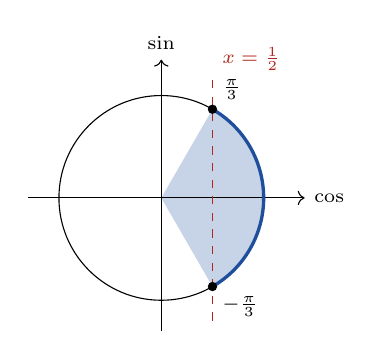
\begin{tikzpicture}[scale=1.3,font=\scriptsize]
\fill[cDef!25] (0,0)--(60:1) arc (60:-60:1)--cycle;
\draw[->] (-1.3,0)--(1.4,0) node[right]{$\cos$}; \draw[->] (0,-1.3)--(0,1.35) node[above]{$\sin$};
\draw (0,0) circle (1); \draw[cDef,very thick] (60:1) arc (60:-60:1);
\draw[cThm,dashed] (0.5,-1.2)--(0.5,1.2); \node[cThm,above right] at (0.5,1.15){$x=\frac12$};
\fill (60:1) circle (1.3pt) node[above right]{$\frac\pi3$}; \fill (-60:1) circle (1.3pt) node[below right]{$-\frac\pi3$};
\end{tikzpicture}\end{LTR}\par مجموعة الحلول $\left[-\frac\pi3;\frac\pi3\right]$.\par}{50 د}{نلون القوس.}
\Row{}{%
\Lab{cEx}{مثال}\ $\sin x>\frac{\sqrt2}2$ في $[0;2\pi[$: $\left]\frac\pi4;\frac{3\pi}4\right[$.\par\Lab{cThm!80!black}{حذار}\ نتبع اتجاه المجال على الدائرة ، وننتبه للأطراف (مغلقة أو مفتوحة).}{}{}
\Row{التقويم}{%
\Lab{cEx}{تطبيق}\par حل: \Num{1} $\cos x<0$ في $]-\pi;\pi]$ ؛ \Num{2} $\sin x\leqslant\frac12$ في $[0;2\pi[$.\par\textbf{الحل:} \Num{1} $\left]-\pi;-\frac\pi2\right[\cup\left]\frac\pi2;\pi\right]$ ؛ \Num{2} $\left[0;\frac\pi6\right]\cup\left[\frac{5\pi}6;2\pi\right[$.\par\textbf{واجب منزلي:} تمارين 89 ، 90 ، 91 من باب الزوايا الموجهة.\par\smallskip\textbf{ملاحظات حول سير الحصة:} \dotfill}{25 د}{نهاية المحور: فرض أو مراجعة.}
\end{Sayr}
\end{document}
